% IEEE Access draft (follow-up paper). Compile with the official IEEE Access LaTeX template
% (ieeeaccess.cls, spotcolor.sty, IEEEtran.bst, logo files) copied into this directory; see paper2/README.md.
% Status: skeleton. System model, analysis, and problem formulation are written; method is outlined;
% setup, results, discussion, and conclusion are placeholders marked \todo{...}.
\documentclass{ieeeaccess}
\usepackage{cite}
\usepackage{amsmath,amssymb,amsfonts}
\usepackage[ruled,linesnumbered]{algorithm2e}
\usepackage{graphicx}
\usepackage{textcomp}
\usepackage{booktabs}
\usepackage{xcolor}
\graphicspath{{figures/}{../paper/}}
\newcommand{\todo}[1]{\textcolor{red}{[TODO: #1]}}

\begin{document}
\history{Date of publication xxxx 00, 0000, date of current version xxxx 00, 0000.}
\doi{10.1109/ACCESS.2026.0000000}

\title{MAPC-Assisted Roaming in IEEE 802.11bn: Coordination Gains in the Mis-Association Window}
\author{\uppercase{Pyoungyun Kim}\authorrefmark{1,2}, \IEEEmembership{Student Member, IEEE}, and \uppercase{Taeyoon Kim}\authorrefmark{3}}
\address[1]{Korea University, 145 Anam-ro, Seongbuk-gu, Seoul 02841, Republic of Korea}
\address[2]{Visual Display Division, Samsung Electronics, Republic of Korea}
\address[3]{School of Mobile System Engineering, Dankook University, Yongin 16890, Republic of Korea}
% Funding statement: none yet. Add \tfootnote{This work was supported by ...} when available.

\markboth
{P. Kim \emph{et al.}: MAPC-Assisted Roaming in IEEE 802.11bn}
{P. Kim \emph{et al.}: MAPC-Assisted Roaming in IEEE 802.11bn}

\corresp{Corresponding author: Taeyoon Kim (e-mail: 2000kty@dankook.ac.kr).}

\begin{abstract}
In dense Wi-Fi deployments, a moving station (STA) remains associated with its access point (AP) for a period after a neighboring AP has become the stronger one, because roaming decisions apply a hysteresis margin, a time-to-trigger, and a received signal strength indicator (RSSI) filter. A small margin shortens this mis-association window but causes the STA to alternate between APs, i.e., AP flapping, whereas a large margin suppresses flapping and prolongs the window. This paper models the mis-association window and the flapping rate of IEEE 802.11 roaming in closed form and quantifies how multi-access point coordination (MAPC) in IEEE 802.11bn changes this trade-off: during the window, the stronger AP stays silent or yields the transmission opportunity, which recovers part of the throughput lost to mis-association. \todo{Main quantitative results: recovered share of the mis-association loss, shift of the optimal hysteresis margin, reduction of the flapping rate, and the gap of learned schedulers to an exact association-aware oracle.}
\end{abstract}

\begin{keywords}
IEEE 802.11bn, multi-access point coordination, roaming, handover hysteresis, AP flapping, mobility, multi-agent reinforcement learning, Wi-Fi 8.
\end{keywords}

\titlepgskip=-21pt

\maketitle

\section{Introduction}
\label{sec:introduction}
\PARstart{A}{} station (STA) that walks through a dense Wi-Fi deployment crosses the coverage boundaries of several access points (APs). In IEEE 802.11, the STA and not the network decides when to roam, and it does so from filtered measurements of the received signal strength indicator (RSSI)~\todo{cite IEEE 802.11 roaming / 802.11k, v, r overview}. To avoid oscillation, the decision applies a hysteresis margin and a time-to-trigger, and many STAs start to scan only after the RSSI of the serving AP falls below a roaming threshold. The STA therefore remains associated with its AP for a period after a neighboring AP has become the stronger one. During this mis-association window, the serving link is weak and the stronger AP is the dominant interferer.

The roaming parameters set a trade-off. A small hysteresis margin shortens the mis-association window, but RSSI fluctuations near the boundary then trigger repeated handovers between the same APs, i.e., AP flapping, and every handover interrupts the service for the duration of the reassociation. A large margin suppresses flapping and prolongs the mis-association window. Cellular networks face the same trade-off as the ping-pong problem~\todo{cite cellular handover hysteresis / TTT / ping-pong studies}.

IEEE 802.11bn, the amendment that defines Wi-Fi~8 with the target of ultra high reliability (UHR), introduces multi-access point coordination (MAPC)~\cite{galati2024wifi8}. Under MAPC, neighboring APs share a transmission opportunity (TXOP) in time, as in coordinated time division multiple access (Co-TDMA), or in space, as in coordinated spatial reuse (Co-SR)~\cite{lopez2019ieee}. MAPC acts directly on the mis-association window: the stronger AP stays silent or yields the TXOP while the weaker serving AP reaches the STA. MAPC therefore lowers the cost of a large hysteresis margin and shifts the roaming trade-off.

This paper quantifies that shift. The contributions are as follows.
\begin{itemize}
\item A model of STA mobility, filtered RSSI measurement, hysteresis-based roaming, handover interruption, and queue transfer, integrated with the MAPC scheduling model of~\todo{cite companion paper (exact-oracle gap analysis)}.
\item Closed-form expressions for the length of the mis-association window and an approximation of the flapping rate as functions of the hysteresis margin, the time-to-trigger, the RSSI filter, the AP spacing, and the STA speed.
\item An exact association-aware per-slot oracle, an ideal-association upper bound, and a finite-horizon oracle with a switching cost, which separate the loss caused by roaming delay from the loss caused by scheduling.
\item A quantitative evaluation of the share of the mis-association loss that MAPC recovers and of the resulting shift of the optimal roaming parameters, for Co-TDMA, exact scheduling, and learned schedulers with centralized training and decentralized execution (CTDE).
\end{itemize}

The remainder of the paper is organized as follows. Section~\ref{sec:related} reviews related work. Section~\ref{sec:system} defines the system model, Section~\ref{sec:analysis} analyzes the mis-association window and the flapping rate, and Section~\ref{sec:problem} formulates the scheduling problem. Section~\ref{sec:method} presents the reference schedulers and the learners, Section~\ref{sec:setup} details the experimental setup, Section~\ref{sec:results} reports the results, Section~\ref{sec:discussion} discusses design implications, and Section~\ref{sec:conclusion} concludes the paper.

\section{Related Work}
\label{sec:related}
\subsection{Roaming in IEEE 802.11}
\todo{IEEE 802.11k (neighbor reports), 802.11v (BSS transition management), 802.11r (fast BSS transition); sticky-client behavior; measured handover latency of legacy and fast transition. Every citation verified against a primary record before it enters references.bib.}

\subsection{Handover hysteresis and ping-pong}
\todo{Cellular A3-event handover with hysteresis and time-to-trigger; analytical ping-pong models; mobility models, including the Gauss--Markov model.}

\subsection{MAPC and learned scheduling}
MAPC is a core feature of IEEE 802.11bn~\cite{galati2024wifi8,lopez2019ieee}, and analytical studies quantify the throughput gain of Co-SR over uncoordinated access~\cite{wilhelmi2023csr}. Learned MAPC schedulers include proximal policy optimization (PPO) agents~\cite{nunez2026drl} and machine-learning-based Co-SR scheduling~\cite{wojnar2025csr}; surveys cover machine learning for Wi-Fi more broadly~\cite{szott2022wifiml}. These works assume a fixed association between STAs and APs. \todo{Seamless roaming in IEEE 802.11bn: cite the primary source once verified.}

\section{System Model}
\label{sec:system}
\subsection{Network and mobility}
The network consists of $N$ APs indexed by $i \in \mathcal{N} = \{1,\dots,N\}$ at fixed positions $\mathbf{p}_i \in \mathbb{R}^2$ and $M$ STAs indexed by $k \in \mathcal{K} = \{1,\dots,M\}$. Time is divided into scheduling slots of duration $T_{\text{slot}} = 1$~ms. STA $k$ moves according to the Gauss--Markov mobility model
\begin{equation}
\mathbf{v}_k(t) = \beta\,\mathbf{v}_k(t-1) + (1-\beta)\,\bar{\mathbf{v}}_k + \sqrt{1-\beta^2}\,\sigma_v\,\mathbf{w}_k(t),
\label{eq:velocity}
\end{equation}
\begin{equation}
\mathbf{x}_k(t+1) = \mathbf{x}_k(t) + T_{\text{slot}}\,\mathbf{v}_k(t),
\label{eq:position}
\end{equation}
where $\mathbf{x}_k(t)$ and $\mathbf{v}_k(t)$ are the position and velocity of STA $k$, $\beta \in [0,1]$ is the memory parameter, $\bar{\mathbf{v}}_k$ is the mean velocity, $\sigma_v$ is the velocity standard deviation, and $\mathbf{w}_k(t)$ is a standard bivariate Gaussian vector. The distance between AP $i$ and STA $k$ is $d_{i,k}(t) = \|\mathbf{p}_i - \mathbf{x}_k(t)\|$, and the received power follows the indoor path-loss model
\begin{equation}
P_{\text{rx}}(d) = P_{\text{tx}} - 46.67 - 30 \log_{10} \max(d, 1) \quad [\text{dBm}],
\label{eq:pathloss}
\end{equation}
with transmit power $P_{\text{tx}} = 15$~dBm and noise power $P_{\text{N}} = -95$~dBm.

\subsection{RSSI measurement and filtering}
In slot $t$, STA $k$ measures the RSSI of AP $i$ as
\begin{equation}
R_{i,k}(t) = P_{\text{rx}}\bigl(d_{i,k}(t)\bigr) + X_{i,k}(t),
\label{eq:rssi}
\end{equation}
where $X_{i,k}(t)$ is a zero-mean measurement deviation with standard deviation $\sigma_X$ in dB that represents small-scale fading. The STA filters the measurements with an exponential moving average,
\begin{equation}
\bar{R}_{i,k}(t) = (1-\alpha)\,\bar{R}_{i,k}(t-1) + \alpha\,R_{i,k}(t),
\label{eq:filter}
\end{equation}
where $\alpha \in (0, 1]$ is the filter coefficient.

\subsection{Association and roaming}
The association of STA $k$ in slot $t$ is $a_k(t) \in \mathcal{N}$. STA $k$ hands over from AP $a_k(t)$ to AP $j \ne a_k(t)$ when the two conditions
\begin{equation}
\bar{R}_{j,k}(s) > \bar{R}_{a_k(t),k}(s) + \Delta_{\text{hys}} \quad \text{and} \quad \bar{R}_{a_k(t),k}(s) < R_{\text{roam}}
\label{eq:roam}
\end{equation}
hold in every slot $s \in \{t - n_{\text{TTT}} + 1, \dots, t\}$, where $\Delta_{\text{hys}} \ge 0$ is the hysteresis margin in dB, $R_{\text{roam}}$ is the roaming threshold in dBm, and $n_{\text{TTT}}$ is the time-to-trigger in slots. When several APs satisfy~\eqref{eq:roam}, the STA selects the one with the largest filtered RSSI. After the trigger, the STA is unreachable for $n_{\text{HO}}$ slots, which model scanning, authentication, and reassociation, and then $a_k$ takes the value $j$.

\subsection{Scheduling and link outcome}
In slot $t$, AP $i$ selects a target $u_i(t) \in \mathcal{S}_i(t) \cup \{\varnothing\}$, where $\mathcal{S}_i(t) = \{k : a_k(t) = i,\ k \text{ reachable}\}$ is the set of reachable STAs associated with AP $i$ and $\varnothing$ denotes silence, and a modulation and coding scheme (MCS) index $m_i(t)$. The set of transmitting APs is $\mathcal{A}(t) = \{i : u_i(t) \ne \varnothing\}$. The signal-to-interference-plus-noise ratio (SINR) of the link from AP $i$ to STA $k = u_i(t)$ is
\begin{equation}
\gamma_{i}(t) = \frac{h_{i,k}(t)\,P_{\text{rx}}\bigl(d_{i,k}(t)\bigr)}{\sum_{j \in \mathcal{A}(t) \setminus \{i\}} h_{j,k}(t)\,P_{\text{rx}}\bigl(d_{j,k}(t)\bigr) + P_{\text{N}}},
\label{eq:sinr}
\end{equation}
where all powers are in linear scale and $h_{j,k}(t)$ is the small-scale fading power gain. MCS $m$ requires an SINR of at least $\theta_m = 2 + 1.5m$~dB and carries $c_m = 1 + \lfloor 1.5 m \rfloor$ packets per slot, as in~\todo{cite companion paper}.

\subsection{Queues and handover}
The downlink queue $q_k(t) \in [0, Q_{\max}]$ of STA $k$ resides at its serving AP. In every slot, $A_k(t) \sim \text{Poisson}(\lambda)$ packets arrive, the backlog after arrivals is $\tilde{q}_k(t) = \min\bigl(q_k(t) + A_k(t), Q_{\max}\bigr)$, and
\begin{equation}
q_k(t+1) = \tilde{q}_k(t) - D_k(t),
\label{eq:queue}
\end{equation}
where $D_k(t) = \mathbb{1}[\gamma_{a_k(t)}(t) \ge \theta_{m}]\min\bigl(\tilde{q}_k(t), c_{m}\bigr)$ for $k = u_{a_k(t)}(t)$ and $m = m_{a_k(t)}(t)$, and $D_k(t) = 0$ otherwise. At a handover, the old AP forwards the backlog to the new AP over the distribution system with a delay of $n_{\text{fwd}}$ slots, or discards it; the forwarding policy is a model parameter.

\section{Analysis of the Mis-Association Window and AP Flapping}
\label{sec:analysis}
\subsection{Length of the mis-association window}
Consider two APs at distance $L$ and a STA that moves from AP~1 toward AP~2 on the line between them at constant speed $v$, with position $x \in (0, L)$ measured from AP~1. Without measurement deviation, the RSSI difference follows from~\eqref{eq:pathloss} as
\begin{equation}
D(x) = \bar{R}_{2}(x) - \bar{R}_{1}(x) = 30 \log_{10}\frac{x}{L - x}.
\label{eq:rssi_difference}
\end{equation}
The boundary of equal RSSI lies at $x = L/2$, and the hysteresis condition $D(x) > \Delta_{\text{hys}}$ first holds at $x_{\Delta}$ with
\begin{equation}
x_{\Delta} - \frac{L}{2} = \frac{L}{2}\tanh\!\left(\frac{\Delta_{\text{hys}} \ln 10}{60}\right).
\label{eq:hysteresis_distance}
\end{equation}
The roaming threshold condition holds beyond $x_{\text{roam}} = 10^{(P_{\text{tx}} - 46.67 - R_{\text{roam}})/30}$. The mis-association window, i.e., the time during which AP~2 is the stronger AP while the STA is associated with AP~1 or is unreachable, therefore lasts
\begin{equation}
T_{\text{MA}} = \frac{\max(x_{\Delta}, x_{\text{roam}}) - L/2}{v} + (n_{\text{TTT}} + n_{\text{HO}})\,T_{\text{slot}}.
\label{eq:window}
\end{equation}
For $L = 20$~m and $\Delta_{\text{hys}} = 3$~dB, \eqref{eq:hysteresis_distance} gives 1.15~m, i.e., 1.15~s at a walking speed of 1~m/s, which is about 5.7 times the episode length of 200 slots used in~\todo{cite companion paper}.

\subsection{Flapping rate}
Near the boundary, the filtered RSSI difference is $D_k(t) = \mu_k(t) + \varepsilon_k(t)$, where $\mu_k(t)$ is the deterministic difference~\eqref{eq:rssi_difference} at the current position and $\varepsilon_k(t)$ is the difference of the two filtered measurement deviations. For deviations that are independent across slots and APs, the stationary variance of $\varepsilon_k(t)$ under~\eqref{eq:filter} is
\begin{equation}
\sigma_{\varepsilon}^2 = \frac{2\alpha}{2-\alpha}\,\sigma_X^2,
\label{eq:filtered_variance}
\end{equation}
and its lag-one correlation coefficient is $1 - \alpha$. The probability that the hysteresis condition holds in a given slot is $Q\bigl((\Delta_{\text{hys}} - \mu_k)/\sigma_{\varepsilon}\bigr)$, where $Q(\cdot)$ is the Gaussian tail function, and this value bounds the per-slot trigger probability $p_{\text{HO}}$ from above for every $n_{\text{TTT}} \ge 1$. At the boundary, $\mu_k = 0$, and the association evolves as a two-state Markov chain with symmetric transition probability $p_{\text{HO}}$ per slot. Under the approximation of independent triggers, the dwell time in one AP is geometric with mean $1/p_{\text{HO}}$ slots, and the probability that the STA returns to the previous AP within $n_{\text{pp}}$ slots, which defines a flapping event, is
\begin{equation}
P_{\text{flap}} = 1 - (1 - p_{\text{HO}})^{n_{\text{pp}}}.
\label{eq:flap}
\end{equation}
The exact trigger probability with filter correlation and $n_{\text{TTT}} > 1$ is obtained by simulation.

\subsection{Throughput loss of roaming}
The throughput loss of roaming per boundary crossing is
\begin{equation}
L_{\text{roam}} = \underbrace{T_{\text{MA}}\,\bigl(\rho^{\star}_{\text{ideal}} - \rho^{\star}_{\text{MA}}\bigr)}_{\text{mis-association}} + \underbrace{N_{\text{HO}}\,\bigl(n_{\text{HO}}\,T_{\text{slot}}\,\rho^{\star}_{\text{ideal}} + B_{\text{fwd}}\bigr)}_{\text{handover and flapping}},
\label{eq:roam_loss}
\end{equation}
where $\rho^{\star}_{\text{ideal}}$ and $\rho^{\star}_{\text{MA}}$ are the service rates of the STA under ideal association and during mis-association, $N_{\text{HO}}$ is the number of handovers per crossing including flapping, and $B_{\text{fwd}}$ is the backlog lost or delayed at each handover. A larger $\Delta_{\text{hys}}$ increases the first term and decreases the second. MAPC raises $\rho^{\star}_{\text{MA}}$, because the stronger AP stays silent or yields the TXOP during the window, and thereby lowers the first term for every $\Delta_{\text{hys}}$.

\section{Problem Formulation}
\label{sec:problem}
The slot throughput is $R(t) = \sum_{k \in \mathcal{K}} D_k(t)$. For a given roaming policy, i.e., a given tuple $(\Delta_{\text{hys}}, n_{\text{TTT}}, \alpha, R_{\text{roam}})$, the scheduling objective over an episode of $T$ slots is
\begin{equation}
J(\pi) = \mathbb{E}_{\pi}\Bigl[\sum_{t=0}^{T-1} R(t)\Bigr],
\label{eq:objective}
\end{equation}
where $\pi$ maps observations to the targets and MCS indices of all APs. The roaming design problem selects the roaming policy that maximizes $\max_{\pi} J(\pi)$ for a scheduler class, e.g., Co-TDMA, exact per-slot scheduling, or a learned CTDE scheduler.

IEEE 802.11bn also considers changing the serving AP of a STA without reassociation. In this variant, the scheduler selects $a_k(t)$ directly, and a switching cost $c_{\text{sw}} \ge 0$ penalizes each change:
\begin{equation}
J_{\text{sw}}(\pi) = \mathbb{E}_{\pi}\Bigl[\sum_{t=0}^{T-1} \Bigl(R(t) - c_{\text{sw}} \sum_{k \in \mathcal{K}} \mathbb{1}\bigl[a_k(t) \ne a_k(t-1)\bigr]\Bigr)\Bigr].
\label{eq:objective_switch}
\end{equation}
The switching cost couples consecutive slots, so a per-slot maximization of~\eqref{eq:objective_switch} does not yield its multi-slot optimum in general.

\section{Reference Schedulers and Learners}
\label{sec:method}
\subsection{Association-aware exact per-slot oracle}
\todo{For a given association $\mathbf{a}(t)$, enumerate all target vectors over $\mathcal{S}_i(t) \cup \{\varnothing\}$ with the highest decodable MCS per link, as in the companion paper; the vectorized implementation in this repository covers $N \le 6$.}

\subsection{Ideal-association upper bound}
\todo{Associate every STA with the AP of largest instantaneous RSSI in every slot, without handover interruption, and apply the per-slot oracle. The difference to the oracle under the roaming policy isolates the roaming loss.}

\subsection{Finite-horizon oracle with switching cost}
\todo{Dynamic programming over association changes within a horizon of $H$ slots for~\eqref{eq:objective_switch}; complexity and the chosen $H$.}

\subsection{Learned schedulers}
\todo{MAPPO with local actors and Central PPO with a full-information actor, as in the companion paper; observation extended with the filtered RSSI of neighboring APs and the association state; action masking of unreachable STAs.}

\section{Experimental Setup}
\label{sec:setup}
\todo{Trajectories: straight crossing between two APs and Gauss--Markov walks in the random topologies of the companion paper. Speed 0.5--2~m/s; $\Delta_{\text{hys}} \in \{0, 1, 3, 6, 10\}$~dB; $n_{\text{TTT}} \in \{0, 40, 160\}$ slots; $\alpha \in \{0.1, 0.5, 1\}$; $R_{\text{roam}} \in \{-65, -70, -75\}$~dBm; $n_{\text{HO}}$ for legacy roaming and fast basic service set (BSS) transition; $\sigma_X$ from the Rayleigh fading statistics; episode length of several seconds; load $\lambda$ above the Co-TDMA capacity.}

\section{Results}
\label{sec:results}
\todo{(a) Mis-association window and flapping rate versus $\Delta_{\text{hys}}$: closed form~\eqref{eq:window}, \eqref{eq:flap} against simulation. (b) Roaming loss~\eqref{eq:roam_loss} without coordination, with Co-TDMA, and with the exact oracle; share of the mis-association loss recovered by MAPC. (c) Optimal $\Delta_{\text{hys}}$ and flapping rate with and without MAPC. (d) Gap of learned schedulers to the association-aware oracle.}

\section{Discussion}
\label{sec:discussion}
\todo{Design guidance for roaming parameters under MAPC; relation to seamless roaming in IEEE 802.11bn; limitations.}

\section{Conclusion}
\label{sec:conclusion}
\todo{Conclusion.}

% Acknowledgment: none yet. Add \section*{Acknowledgment} here when available.

\bibliographystyle{IEEEtran}
\bibliography{references}

\begin{biography}[{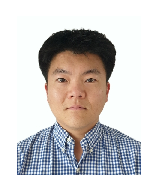
\includegraphics[width=1in,height=1.25in,clip,keepaspectratio]{photo/kpy.eps}}]{Pyoungyun Kim} (S'25)
received the B.S. and M.S. degrees from Korea University, Seoul, Korea, in 2005 and 2007, respectively. Since 2007, he has been with Samsung Electronics, where he has contributed to smart recommendation agents, the integration of the Consumer Electronics Control (CEC) protocol into television systems, and Tizen-based TV software applications. He is currently a Senior Engineer with the Product S/W Lab, Visual Display Division, Samsung Electronics, where he works on multi-view features for smart TVs and screen control for projectors. His research interests include on-device artificial intelligence (AI) for smart displays, embedded deep learning optimization, and resource-efficient deep reinforcement learning (DRL).
\end{biography}

\begin{biography}[{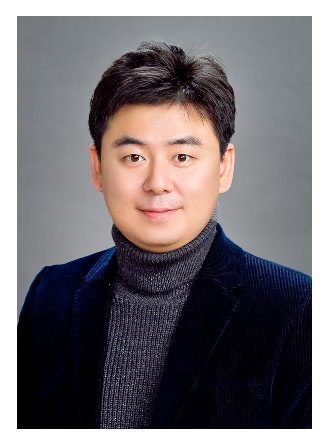
\includegraphics[width=1in,height=1.25in,clip,keepaspectratio]{photo/kty.eps}}]{Taeyoon Kim}
received the B.S., M.S., and Ph.D. degrees in electronics and computer engineering from Korea University in 2005, 2007, and 2019, respectively. He was a Research Engineer with Hyundai Motors from 2007 to 2010 and an Assistant Professor with Soonchunhyang University from 2019 to 2021. In 2021, he joined Dankook University as an Assistant Professor with the School of Mobile System Engineering. He was a Visiting Researcher with the University of British Columbia in 2017. His research interests include network architectures and protocols for next-generation networks, such as WLAN, 5G, and time-sensitive networking (TSN), and AI-enabled edge intelligence.
\end{biography}

\EOD

\end{document}
